\chapter{Das Metaverse}\label{ch:Metaverse}

\section{Definitionen und Konzept}

Der Begriff \glqq Metaverse\grqq{} wurde erstmals in dem 1992 erschienen Science-Fiction-Roman \glqq Snow Crash\grqq{} von Neal Stephenson erwähnt und wird dort als virtuelle Welt dargestellt, in die sich die Protagonisten als digitale Repräsentation, so genannte \glqq Avatare\grqq{} flüchten (vgl. \cite{DripSnow},\cite{MVkompaktSnow}). Dieses Metaverse stellte eine dauerhafte virtuelle Welt dar, die nahezu alle Aspekte des menschlichen Lebens umfasste, mit ihnen interagierte und sie beeinflusste. Bereist vorher gab es vereinzelte Werke von anderen Autoren, die einzelne Aspekte des Metaverse beinhalteten. Das Metaverse, wie es geplant ist oder in der Vorstellung existieren soll, ist derzeit noch nicht realisiert. Bislang gibt es lediglich vereinzelte \glqq Metawelten\grqq{} oder \glqq Metagalaxien\grqq{}, die einzelne Charakteristika (siehe Abbildung \ref*{fig:CharakteristikadesMV}) des Metaverse abdecken und damit eine Proto-Metaverse erstellen. 

Untersucht man die etymologische, also die herkunftsbezogene, Bedeutung des Begriffs, setzt sich Metaverse (auch Metaversum) aus dem griechischen Präfix\glqq meta\grqq{} (über) und \glqq verse\grqq{} bzw. \glqq versum\grqq{} (universe/universum) zusammen. Es handelt sich demnach um ein Über-Universum, das jenseits der analogen Welt liegt. Für den Begriff Metaverse findet sich jedoch zum aktuellen Zeitpunkt noch keine einheitliche Definition. Jedoch sind viele Definitionen im Umlauf.

Satya Nadella, der CEO von Microsoft beschreibt das Metaverse so: \glqq Mit der Konvergenz von virtueller und physischer Welt entwickelt sich das Metaversum, das aus digitalen Zwillingen, simulierten Umgebungen und gemischter Realität besteht, zu einer erstklassigen Plattform. Mit dem Metaverse wird die gesamte Welt zur Leinwand für Ihre App.\grqq{} \cite[frei übersetzt]{MicDef}

Definition des Metaverse vom Bundesverband Digitale Wirtschaft: \glqq Die ultimative Vision des Metaverse ist ein dezentralisiertes, interoperables, beständiges und mit allen Sinnen wahrnehmbares, digitales Ökosystem mit unbegrenzter Nutzerkapazität. Es wird sowohl in einer erweiterten (AR) als auch in einer rein virtuellen Realität (VR) mit der physischen Welt koexistieren. Das voll entwickelte Metaverse wird mit dem realen Leben verschmelzen und unsere Gesellschaft und die Art und Weise, wie wir uns vernetzen, miteinander arbeiten, leben und mit Marken interagieren, grundlegend verändern. \grqq{} \cite{BVDWDef}

Matthew Ball beschreibt das Metaverse als \glqq Ein massiv skaliertes und interoperables Netzwerk von in Echtzeit gerenderten virtuellen 3D-Welten, die synchron und dauerhaft von einer praktisch unbegrenzten Anzahl von Nutzern mit einem individuellen Gefühl der Präsenz und mit einer Kontinuität der Daten wie Identität, Geschichte, Berechtigungen, Objekte, Kommunikation und Zahlungen erlebt werden können.\grqq{} \cite{Ball22Def}

Weitere Definitionen finden sich in \glqq Metaverse kompakt\grqq{} von Ralf T. Kreutzer und Sonja Klose. Anhand dieser verschiedenen Definitionen wurden die in Abbildung \ref{fig:CharakteristikadesMV} dargestellten Charakteristika des Metaverse ermittelt, die im Folgenden näher erläutert werden. (Vgl. \cite{MVkompaktDef})  

\section{Charakteristika des Metaverse}

\begin{figure}[!h]
    \centering
    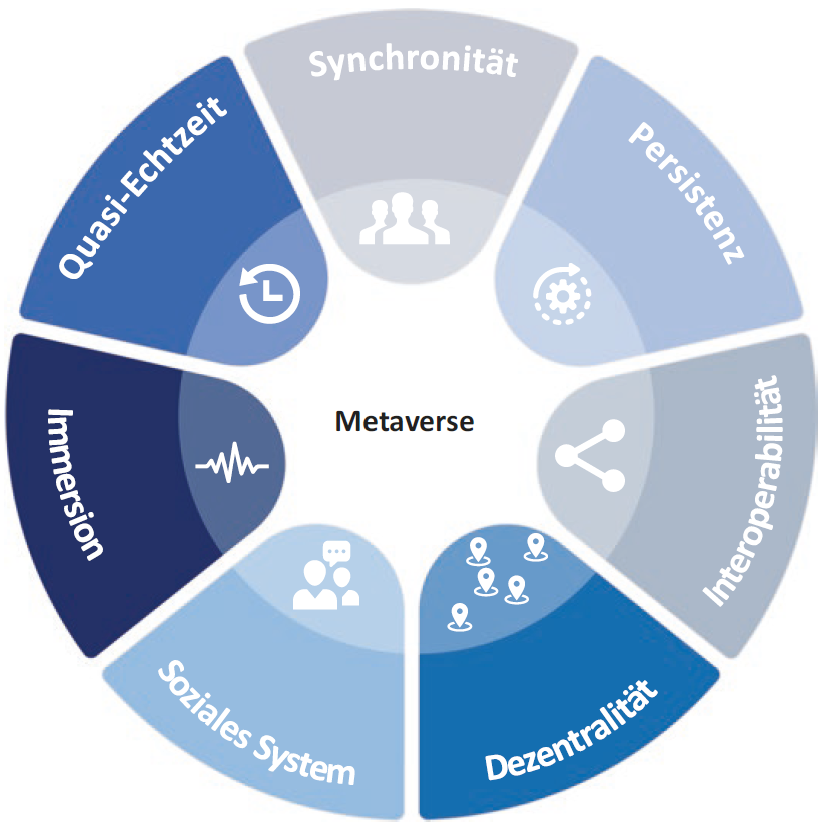
\includegraphics[width = 10cm]{figures/CharakteristikadesMV.png}
    \caption{Charakteristika des Metaverse}
    \cite{MVkompaktDef}
    \label{fig:CharakteristikadesMV}
\end{figure}

\paragraph{Immersion:} Der Begriff Immersion beschreibt das \glqq Eintauchen\grqq{} in eine dreidimensionale virtuelle Umgebung oder eine Mischung aus realer und virtueller Welt. Diese virtuellen Umgebungen können sowohl reale Orte als auch fiktive Versionen realer Umgebungen oder vollständig erfundene Welten darstellen. Wenn reale Umgebungen abgebildet werden, spricht man meist von Digitalen Zwillingen. (vgl. \cite{Ball22charak}, \cite{MVkompaktCharak})

\paragraph{Soziales System} Das Metaverse ist ein soziales System, in dem Menschen sich begegnen und sowohl miteinander als auch mit Organisationen interagieren können. Da der Mensch ein soziales Wesen ist, soll das Metaverse nicht nur Arbeits- und Spielmöglichkeiten bieten, sondern auch die Möglichkeit, Freundschaften zu schließen, Liebesbeziehungen zu führen, Sexualität auszuleben und andere menschliche Bedürfnisse zu erfüllen. (vgl. \cite{MVkompaktCharak})

\paragraph{Quasi-Echtzeit:} Da eine vollständig latenzfreie Übertragung mit dem aktuellen Stand der Technik nicht möglich ist, soll die ortsunabhängige Interaktivität in Quasi-Echtzeit erfolgen. Für immersive Erfahrungen ist es nachteilig, wenn eine niedrige Bandbreite oder zu hohe Latenz die Sinneseindrücke der virtuellen Umgebung beeinträchtigen. (vgl. \cite{Ball22charak})

\paragraph{Persistenz:} Mit Persistenz wird beschrieben, dass das Metaverse und die persönliche Account-Historie unabhängig von einzelnen oder mehreren Unternehmen dauerhaft bestehen bleiben. Die virtuellen Welten im Metaverse sollen sich weiterentwickeln und Veränderungen in ihnen dauerhaft für jeden Akteur erhalten bleiben, selbst wenn sich niemand innerhalb dieser Welt aufhält. (vgl. \cite{persist},\cite{MVkompaktCharak}) 

\paragraph{Synchronität:} Synchronität bedeutet dass eine unbegrenzte Anzahl von Benutzern gleichzeitig in den virtuellen Welten interagieren kann. Das Metaverse soll ein Ort der sozialen Interaktion sein, was vorraussetzt das die Beteiligten parallel agieren können. Dies benötigt jedoch eine unbegrenzte Kapazität an Verfügbarkeit von Zugangspunkten, Anmeldeservern und Speicher für die benutzerspezifischen Daten. (vgl. \cite{BVDWDef}) 

\paragraph{Interoperabilität:} Daten- und geräteübergreifende Interoperabilität bedeutet, dass virtuelle Inhalte auf verschiedenen Plattformen genutzt werden können. Die Geräte, die für den Zugriff auf das Metaverse benötigt werden, sollten ebenfalls plattformunabhängig einsetzbar sein. Auch die virtuelle Identität soll plattformübergreifend nutzbar sein, vergleichbar mit Pässen, Sozialversicherungsnummern oder anderen nationalen Identifikationsmitteln. Dafür sind gemeinsame Standards erforderlich.

\paragraph{Dezentralität: } Bei der Dezentralität herscht Uneinigkeit ob es ein Charakteristikum des Metaverse ist oder eine reine Komponente des Web 3.0. (vgl. \cite{Ball22charak}) Im Kontext des Metaverse bedeutet Dezentralität die Verlagerung von Kontrolle und Entscheidungsfindung von einer zentralisierten Einheit, wie einer Einzelperson oder Organisation, auf ein verteiltes Netzwerk. Dadurch wird sichergestellt, dass keine einzelne Instanz Autorität oder Kontrolle über andere ausübt. (vgl. \cite{Ball22charak}, \cite{MVkompaktCharak})


(vgl. \cite{Ball22charak}, \cite{MVkompaktCharak})

\section{Technologien im Metaverse}


\subsection{Extended Reality (XR)}

Für das Eintauchen in virtuelle Welten ist der Besitz technischer Hardware erforderlich, die dies ermöglicht. Im Vordergrund stehen die Technologien Virtual Reality (VR) und Augmented Reality (AR), die zusammen unter dem Begriff Extended Reality (XR) bekannt sind.

Bei VR wird die physische Welt vollständig ausgeblendet, sodass der Nutzer vollständig in die virtuelle Welt eintaucht. Dies ermöglicht den höchsten Grad an Immersion.

Bei AR werden virtuelle Inhalte in die physische Welt projiziert, sodass der Nutzer sie betrachten und mit ihnen interagieren kann.

Beide Technologien funktionieren über Headsets, Brillen und im Fall von AR sogar über Kontaktlinsen. (vgl. \cite{XR-DM})

Eine weitere Möglichkeit besteht im Einsatz von LEDs, die auf flexible, magnetische Panels montiert und auf Unterkonstruktionen befestigt werden können. Diese Panels lassen sich in unterschiedliche Formen bringen. Zudem sind auch LED-Böden realisierbar, die mehrere Tonnen pro Quadratmeter tragen können. Auf diese Weise können ganze Räume oder Bereiche in eine virtuelle Welt verwandelt werden.

\begin{figure}[!h]
    \centering
    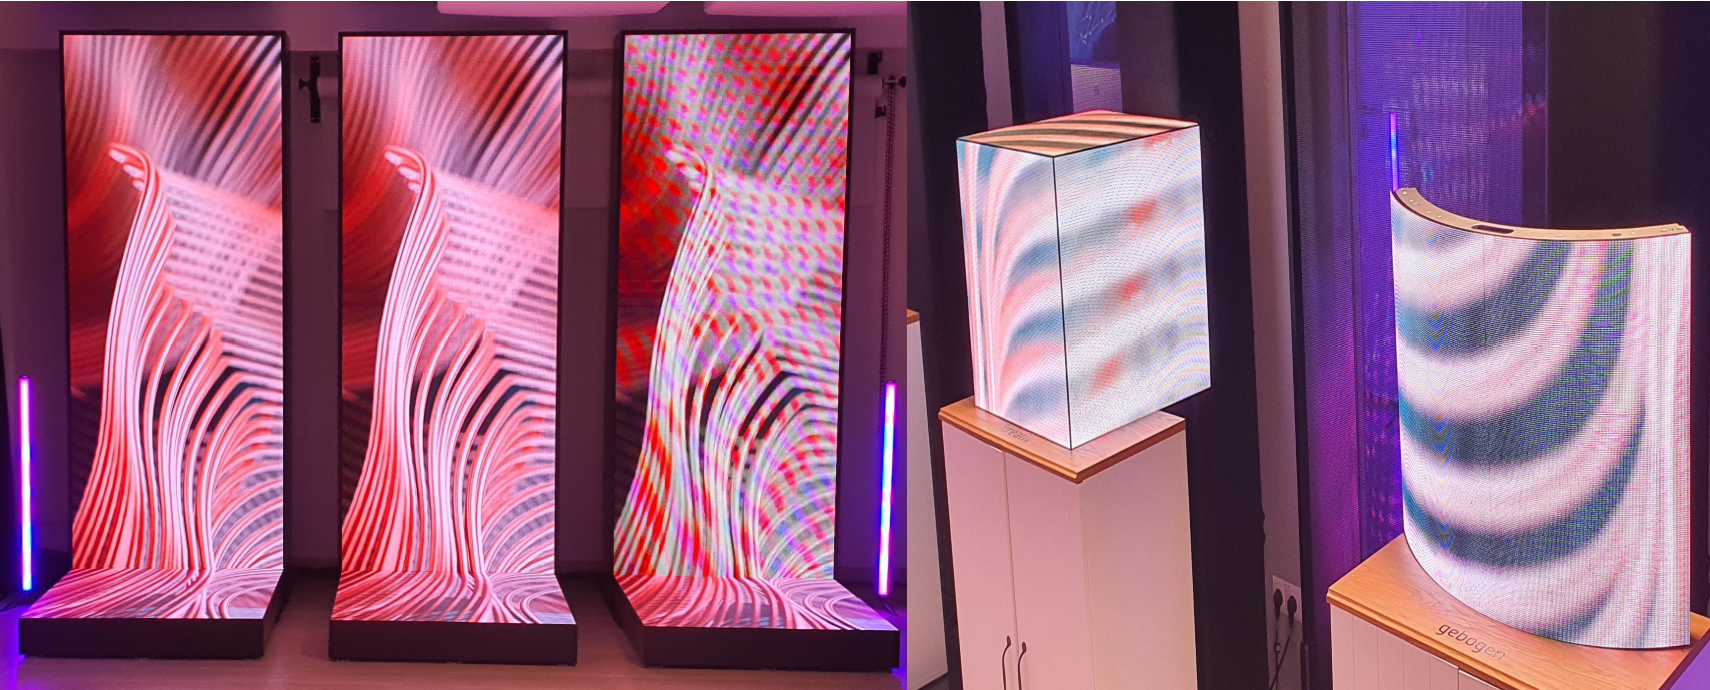
\includegraphics[width = 10cm]{figures/LEDs.png}
    \caption{LEDs präsentiert auf der PAVE Experience Week 2024}
    \label{fig:PaveLED}
\end{figure}

Auch normale Computerbildschirme können genutzt werden, erreichen jedoch nur einen niedrigen Grad der Immersion. 

\subsection{Künstliche Intelligenz}

Künstliche Intelligenz (KI) beschäftigt sich damit, wie ein Computer intelligentes, menschliches Verhalten nachahmen kann. KI ist keine einzelne Technologie, sondern setzt sich aus drei wesentlichen Bausteinen zusammen: Daten und Datenbanken, maschinelles Lernen sowie neuronale Netze bzw. analytische Modelle (vgl. \cite{MVkompaktKI}). Künstliche Intelligenz umfasst verschiedene Einsatzgebiete (siehe Abbildung \ref*{fig:KIEInsatzfelder}) und spielt eine zentrale Rolle bei der Entwicklung des Metaverse. 

\begin{figure}[h]
    \centering
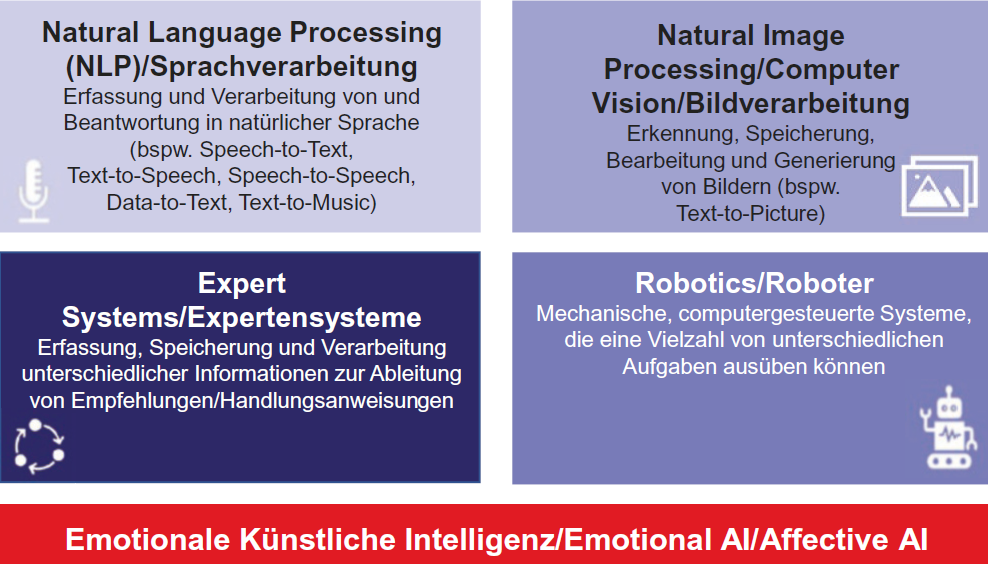
\includegraphics[width = 12cm]{figures/KIEInsatzfelder.png}
\caption{Einsatzfelder der Künstlichen Intelligenz}
\cite{KI}
\label{fig:KIEInsatzfelder}
\end{figure}

KI ermöglicht personalisierte und immersive Erlebnisse, indem sie dynamische virtuelle Welten erschafft und intelligente Avatare erzeugt. So können Personen durch Anwendungen oder Avatarscanner (siehe Abbildung \ref*{fig:ChatBotAvatar}) mithilfe von KI realistische oder abstrakte Avatare von sich selbst erzeugen. Über Programme wie Chat-GPT oder ähnlichen Anwendungen können solche Avatare Fragen beantworten, Gespräche führen oder Aufgaben erledigen.

\begin{figure}[h]
    \centering
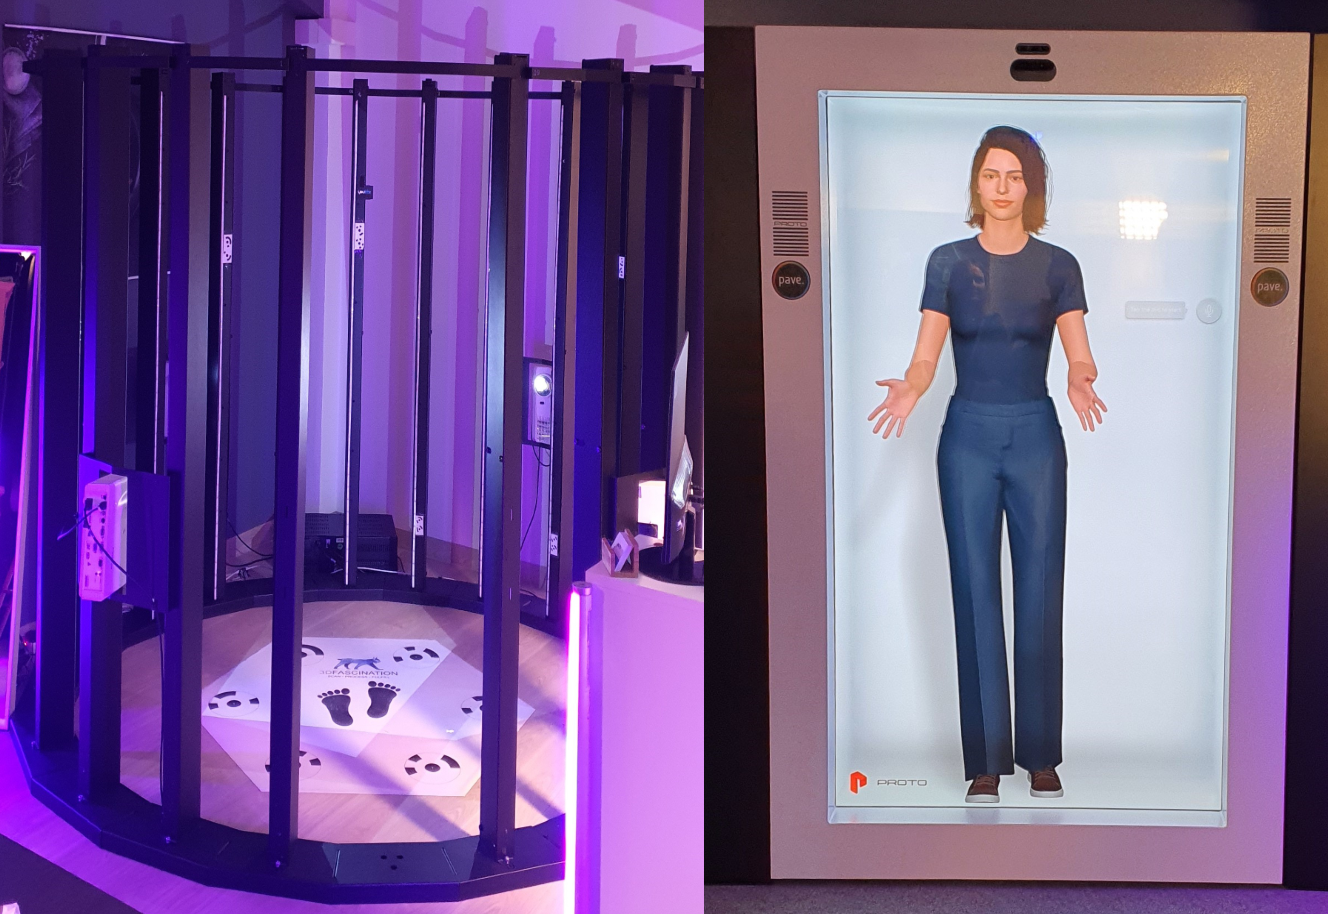
\includegraphics[width = 7cm]{figures/holoAV.png}
\caption{Avatarscanner li. und Hologram Bildschirm re. präsentiert auf der PAVE Experience Week 2024}
\label{fig:ChatBotAvatar}
\end{figure}


\subsection{Blockchain}
Blockchains sind die bekannteste Form der Distributed-Ledger-Technologie (DLT). Der Name leitet sich von ihrer speziellen Struktur ab, bei der Datenblöcke kryptografisch miteinander verkettet werden. Diese Blöcke sind in chronologischer Reihenfolge angeordnet und durch Prüfsummen, sogenannte Hashes, miteinander verknüpft. Sobald ein Datenblock in die Blockchain aufgenommen und der nächste Block angehängt wurde, können die Daten im vorherigen Block nicht mehr verändert werden. Eine Änderung in einem Datenblock würde den Hashwert dieses Blocks verändern, was wiederum den Hashwert des nachfolgenden Blocks beeinflussen würde. Selbst die geringste Änderung, wie das Ändern eines einzigen Zeichens, würde die gesamte nachfolgende Blockkette ungültig machen.(vgl. \cite{Blockchain})

\subsubsection{verteiltes Kontobuch}
Die Technologie, auf der Blockchains basieren, wird als Distributed-Ledger-Technologie (\glqq Technik der verteilten Buchführung\grqq{}) bezeichnet. (vgl. \cite{DripDLT}) Ein DLT beschreibt ein Netzwerk, in dem Daten dezentral organisiert sind. Diese Daten und ihre Transaktionshistorie werden parallel bei allen Netzwerkteilnehmern gespeichert und durch ein Konsensverfahren verifiziert. Dadurch gibt es, anders als bei herkömmlichen Datenbanken, keine zentrale Autorität. Aufgrund dieser Dezentralität gelten die Daten als weitestgehend fälschungssicher und nachvollziehbar. Die Stabilität des Systems bleibt dabei unabhängig von einzelnen Netzwerkteilnehmern gewährleistet. (vgl. \cite{Blockchain})

\subsubsection{Bitcoin}
Die erste populäre Blockchain, Bitcoin, wurde 2009 eingeführt und hat das primäre Ziel, ihre eigene Kryptowährung, Bitcoin, zu betreiben. Sie ermöglicht dezentrale und öffentliche Transaktionen zwischen einander fremden Parteien, ohne dass es zur doppelten Ausgabe derselben Münzen kommen kann. Der Austausch erfolgt über eine Empfangsadresse, die einem öffentlichen Schlüssel entspricht und durch einen kryptografisch verknüpften privaten Schlüssel signiert wird. Dieser private Schlüssel wird in einem Wallet hinterlegt. Dieses Wallet kann ein einfaches Blatt Papier sein, auf dem der Schlüssel notiert ist, eine Hardware, die offline betrieben wird, oder ein Online-Krypto-Wallet. (vgl. \cite{Blockchain}, \cite{BTC})

\subsubsection{Ethereum}

Bitcoin ist mit Abstand die Kryptowährung mit der höchsten Marktkapitalisierung. Auf dem zweiten Paltz folgt Ethereum. \cite{MarketCap} Die Ethereum-Blockchain bietet den Vorteil, dass neben dem Betrieb der eigenen Kryptowährung Ether auch Software darauf gespeichert und ausgeführt werden kann. (vgl. \cite{Blockchain}) 


\subsubsection{Smart-Contracts und NFTs}
\glqq Als Smart Contracts werden Programme auf der Blockchain bezeichnet, die auf Basis einer WENN-DANN-Logik arbeiten, sodass bei Eintritt eines zuvor festgelegten Ereignisses (sog. trigger) automatisch eine ebenfalls zuvor festgelegte Aktion (bspw. eine Transaktion) ausgeführt wird.\grqq{} \cite{SmartConDef}


\subsection{DAPPS und DAO}

Die Blockchain-Technologie ermöglicht den Besitz und die Interoperabilität digitaler Vermögenswerte und schafft so die Grundlage für eine digitale Wirtschaft im Metaverse. Dadurch können Kauf, Verkauf und andere finanzielle Anwendungsfälle realisiert werden, während die Vermögenswerte in verschiedenen Metaverse-Welten genutzt werden können. (Vgl. \cite{tech})
\section{Metawelten und Metagalaxien}




\subsection{Meta}
\subsection{Sandbox}
\subsection{Roblox}
\subsection{Fortnite}
\subsection{Warframe}
\subsection{BMW}
\subsection{Flughafen Hong Kong}
Nvidia Chefsache Metaverse und https://www.wired.com/story/bmw-virtual-factory-ai-hone-assembly-line/